\newpage
\subsection{Arbeitspaket von Herrn Dück$^4$}

Dieser Abschnitt beschreibt, wie Herr Dück die ihm zugeteilten Arbeitspakete bearbeitet und gelöst hat. Darunter fällt die Erstellung einer CSS-Datei für mobile Systeme, die Bewertung von Artikeln sowie die Gestaltung der Bestätigungs-E-Mail.


\subsubsection{Arbeitspaket 2: Die CSS-Datei für die Darstellung auf mobilen Geräten}

\textbf{Warum eine CSS-Datei für mobile Geräte?}
\\
Der Grund für eine zweite CSS ist der, dass auch auf Smartphones und Tablets die Homepage der GBI eine einfache und benutzerfreundliche Struktur haben soll. Ohne diese wird die Website so klein dargestellt, dass die gesamte Breite auf dem mobilen Gerät dargestellt wird.

\begin{figure}[H]
\begin{center}
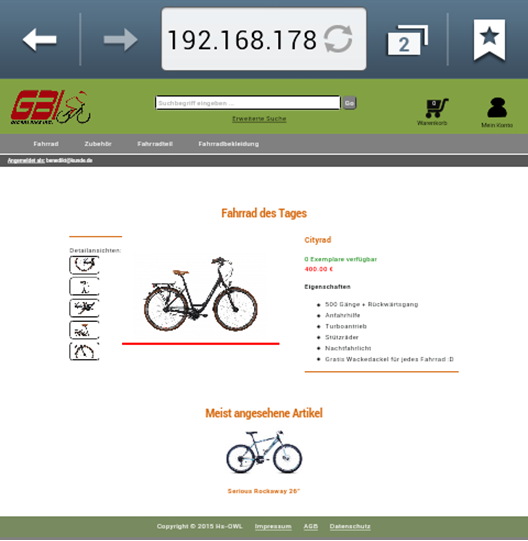
\includegraphics[width=12cm]{Bilder/Michael_Abbildung1-DarstellungDerWebsiteOhneMobileCSS.png}
\end{center}
\caption{Darstellung der Website ohne mobile CSS}
\end{figure}

Mit Tablets wird man damit nicht so große Probleme haben, dennoch muss auch für Tablets das Layout geändert werden. 
Mobile Geräte werden nicht mit einer externen Maus bedient sondern durch eine Touch-Funktion. Das verhindert die Darstellung von Dropdown-Menüs oder Popups durch die CSS-Formatierung ‚hover‘. Dieses Problem wird gelöst, in dem zusätzliche Seiten geschrieben werden, die dann das Dropdown-Menü und Popups ersetzen sollen.

\newpage
\textbf{Layoutgestaltung:}
\\
Zu Beginn der Bearbeitung dieses Paketes musste ein Design der mobilen Ansicht festgelegt werden. Angelehnt an den meisten Webseiten sollte auch hier ein verstecktes Menü eingebaut werden. Bei Klick auf einen Button fährt das Menü vertikal aus bzw. ein. Sowohl die Menüpunkte als auch die Funktionen, die im Header der Website sind, sollten in dieses Dropdown-Menü gelagert werden. Darunter fällt die Suchfunktion, der Zugriff auf den Warenkorb und der Login- bzw. Kontobereich. Der Header wird dementsprechend kleiner. Er enthält nur den Menü-Button und das Logo der GBI.
Formatierungen und Farben wurden größtenteils von der CSS-Datei für Desktop-Geräte übernommen. 
Der Designentwurf für mobile Endgeräte sieht folgendermaßen aus:

	
\begin{figure}[H]
\begin{center}
    \subfigure[Ohne Dropdown-Menü]{
\includegraphics[height=10cm]{Bilder/Michael_Abbildung2-Desingentwurf.png}}
    \subfigure[Mit Dropdown-Menü]{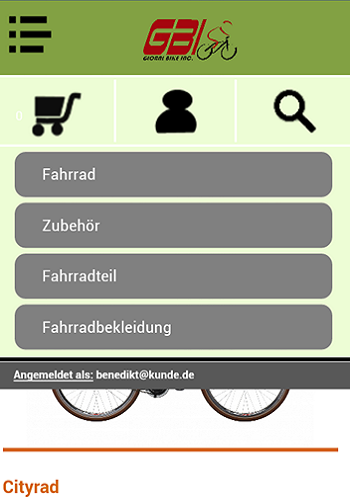
\includegraphics[height=10cm]{Bilder/Michael_Abbildung3-DesingentwurfMitDropDownMenue.png}}
\caption{Designentwurf}
\end{center}
\end{figure}

\textbf{Unterscheidung zwischen Desktop- und mobilen System:}
\\
Zunächst musste die Website beim Öffnen zwischen einen Desktop-System und einem mobilen Gerät unterscheiden können. Dies wird mit folgender Methode gelöst.
\newpage
\begin{center}
	\begin{lstinputlisting}[language=PHP, caption={Unterscheidung Desktop und mobiles Gerät}]
		{Quellcode/Michael-Quellcode1.php}
	\end{lstinputlisting}
\end{center}

Wenn die Methode ‚check\_mobile()‘ den Wert ‚false‘ ausgibt, handelt es sich um Desktop-System. Andern falls ist das Endgerät ein mobiles und zu der schon vorhandenen ‚style.css‘ wird die neue ‚mobile.css‘ importiert. Alle Änderungen, die notwendig für die Darstellung auf einem mobilen Gerät sind, werden hier gespeichert und überschreiben ggf. die Formatierungen in der ‚style.css‘. \\ \\

\textit{Anpassen der Größen:}
\\
Es ist klar, dass die Website, so wie sie  vom ursprünglichen Desktop-Layout erzeugt wird, auf einem Smartphone viel zu klein dargestellt wird, das heißt die komplette Breite der Seite ist im Bild. Um das zu beheben, benötigt es nur eine Zeile in der ‚index.php‘.

\begin{center}
	\begin{lstinputlisting}[language=PHP, caption={Auszug aus der Index-Datei}]
		{Quellcode/Michael-Quellcode2.php}
	\end{lstinputlisting}
\end{center}

Mit diesem Ausdruck wird die Seite auf angenehme Größe heran gezoomt und kann nicht von Benutzer skaliert werden. 
Um das Benutzen der Website praktischer zu gestalten, sollte die Website auf einem mobilen Gerät nur in der vertikalen scrollbar sein. Das gilt sowohl für Handys als auch für Tablets. Im Grunde heißt das, dass die Breite der Website an die Breite des mobilen Gerätes angepasst werden muss. Da in der ‚style.css‘ viel mit Pixel-Breiten gearbeitet wird, bedeutet das, dass alle entsprechenden Elemente umformatiert werden müssen.
Zudem wurden außer Größen auch Anordnungen von Elementen und Farben geändert. Der Grund hierfür ist einfach, das die Website an einigen Stellen zu starke Farben hat und das evtl. unangenehm für den Benutzer werden kann. 



\begin{figure}[H]
\begin{center}
    \subfigure[]{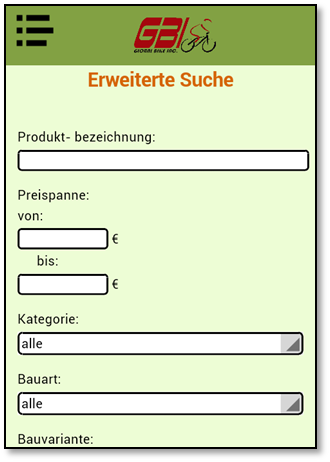
\includegraphics[height=8cm]{Bilder/Michael_Abbildung4-FarbaenderungenFuerBessereLesbarkeit1.png}}
    \subfigure[]{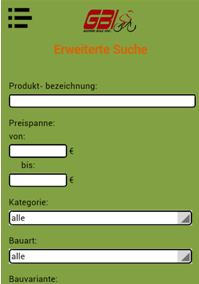
\includegraphics[height=8cm]{Bilder/Michael_Abbildung4-FarbaenderungenFuerBessereLesbarkeit2.png}}
\caption{Farbänderungen für bessere Lesbarkeit}
\end{center}
\end{figure}
\textbf{Menü}
\\
Ein großer Punkt bei der Gestaltung von mobilfähigen Websites ist das Menü. Das Menü kann auf einem Smartphone meist nicht so dargestellt werden, wie es auf der Desktop-Seite der Fall ist. Dort sind alle Menüpunkte in einer Reihe und dafür fehlt der Platz auf mobilen Geräten. Wenn die Menüpunkte untereinander angeordnet werden, ist der Header der Website zu großflächig. Es ist kaum was von dem Inhalt der Seite zu sehen. Aus diesem Grund ist ein Dropdown-Menü genau das richtige. So kann per Druck auf einen Button das Menü aus-, beziehungsweise eingefahren werden. Um den Platz noch sinnvoller zu nutzen, werden die drei Headerfunktionen, die Suche, der Warenkorb und die Kontofunktion, ebenfalls in das Dropdown-Menü versetzt.

\begin{figure}[H]
\begin{center}
    \subfigure[Das Dropdown-Menü]{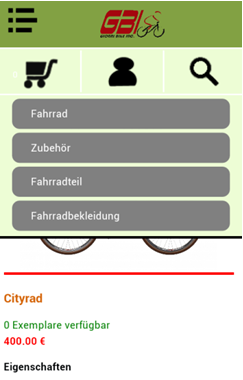
\includegraphics[width=5cm]{Bilder/Michael_Abbildung5-DasDropDownMenue.png}}
    \subfigure[Header mit fester Position]{
\includegraphics[width=5cm]{Bilder/Michael_Abbildung6-HeaderMitFesterPosition.png}}
\caption{Dropdown-Menü und Header}
\end{center}
\end{figure}

Der Header ist auf den Parameter ‚position: fixed‘ eingestellt, das heißt er hat eine festgesetzte Position und verändert sich nicht beim Scrollen der Seite. Das biete den Vorteil, dass das Menü jederzeit sichtbar und schnell erreichbar ist.
\\ \\
\textbf{Neue Seiten:}
\\
Im Laufe der Entwicklung der mobilen CSS wurden mehrere neue Seiten geschrieben. Das liegt daran, dass Funktionen, die auf dem Desktop-System recht praktisch sind, auf mobilen Geräten eher stören. Dazu zählen alle Popups als auch das Untermenü, welches erscheint, wenn man mit der Maus über den Menüpunkt ‚Fahrrad‘ geht. Um trotzdem nicht eingeschränkt zu sein, müssen folgende drei Seiten zusätzlich geschrieben werden:
\begin{enumerate}
\item Die Übersicht der Fahrradkategorien 
\item Eine Login-Seite
\item Eine Übersicht der Kontofunktionen
\end{enumerate}
Die Übersicht der Fahrradkategorien:
\\
Die Übersicht ist tatsächlich nur eine Auflistung aller Fahrradkategorien. Diese erreicht man, wenn der Menüpunkt ‚Fahrrad‘ geklickt wird. 
\\ \\
Eine Login-Seite
\\
Da Popups auf mobilen Geräten nicht angezeigt werden, gibt es sonst keine Möglichkeit sich anzumelden. Deswegen musste eine separate Seite geschrieben werden, auf die man gelangt, wenn man im Menü den Login-Button betätigt. Die Login-Seite bietet ebenfalls eine Weiterleitung zu der Registrierungs-Seite.

\begin{figure}[H]
\begin{center}
    \subfigure[Auflistung der Fahrradkategorien]{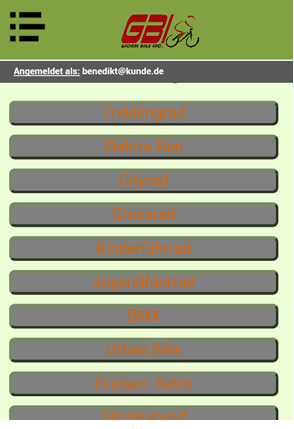
\includegraphics[height=8cm]{Bilder/Michael_Abbildung7-AuflistungDerFahrradkategorien.png}}
    \subfigure[Die Login-Seite]{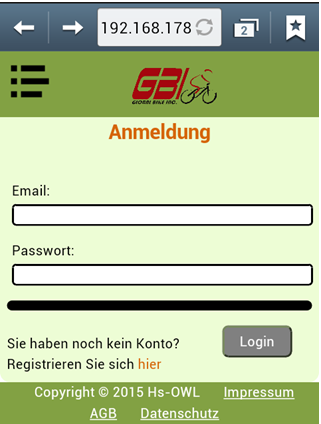
\includegraphics[height=8cm]{Bilder/Michael_Abbildung8-DieLogin-Seite.png}}
\caption{Auflistung der Fahrradkategorien und die Login-Seite}
\end{center}
\end{figure}

Eine Übersicht der Kontofunktionen
\\
Wie im vorherigen Punkt gibt es auch hier keine Möglichkeit, ohne Popup auf die Kontofunktionen zuzugreifen. Die neue Seite ‚(Name der Seite)‘ zeigt eine Übersicht dieser und kann durch Druck auf den Konto-Button erreicht werden.

\begin{figure}[H]
\begin{center}
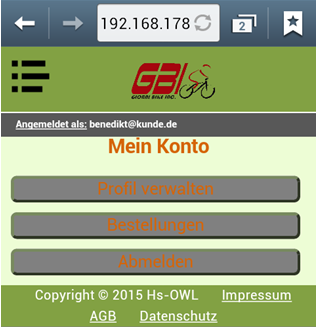
\includegraphics[height=8cm]{Bilder/Michael_Abbildung9-UebersichtDerKontofunktionen.png}
\end{center}
\caption{Übersicht der Kontofunktionen}
\end{figure}

\newpage
\textbf{Probleme/Hindernisse:}
\\
Ein Problem bei der Bearbeitung dieses Arbeitspaketes war die stetige Veränderung der Website, sowohl der PHP-Seiten als auch der CSS-Dateien. Dadurch wurde das Erstellen einer CSS-Datei für mobile Geräte zu einer Langzeitaufgabe, da immer wieder Teile geändert und angepasst werden mussten. 


\subsubsection{Arbeitspaket 11: Die Bewertungsfunktion von Artikeln}

Die Bewertung ist in einem Webshop eine große Hilfe bei der Findung guter Produkte. Deshalb soll diese Funktion in GBI-Webshop auch nicht fehlen. 
In diesem Abschnitt wird alles rund um die Bewertung von Produkten beschrieben. Dabei wird auf das Ansehen und auf das Verfassen einer solchen eingegangen.
\\ \\
Popup zur Bewertung
\\
Um sofort für jeden ersichtlich zu machen, wie ein Artikel bewertet wurde, befindet sich in der Artikelbeschreibung ein Feld mit der Durchschnittlichen Sternebewertung und dahinter eine Angabe, wie viele Bewertungen abgegeben wurden. So kann der Benutzer von vornherein sehen, ob dieser Artikel sich lohnt oder nicht. Will man genau wissen, wie die Aufteilung der Bewertungen auf die Sterne ist, bietet das Feld ein Popupfenster, welches erscheint, wenn man mit der Maus darüber fährt. Zusätzlich befindet sich in diesem Popup ein Link, über den man zu allen Rezensionen dieses Artikels weitergeleitet wird.

\begin{figure}[H]
\begin{center}
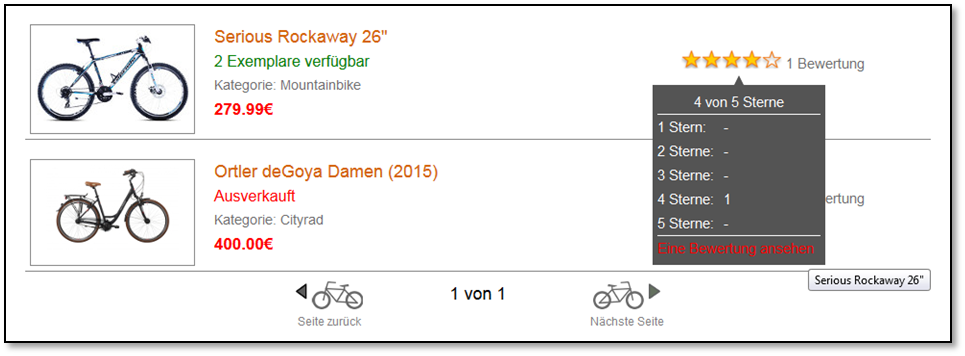
\includegraphics[width=12cm]{Bilder/Michael_Abbildung10-BewertungPopup.png}
\end{center}
\caption{Bewertung Popup}
\end{figure}

Einen Artikel bewerten
\\
Um selber eine Rezension zu diesem Artikel zu verfassen, befindet sich auf der Artikelseite der Link „Artikel bewerten“, über den man zu der Bewertungsseite gelangt. 
Voraussetzung um eine Bewertung abgeben zu können, ist sich zuvor angemeldet zu haben. Ist das nicht der Fall, soll auf die Login-Seite weitergeleitet werden mit einem Hinweis sich anzumelden.

\begin{figure}[H]
\begin{center}
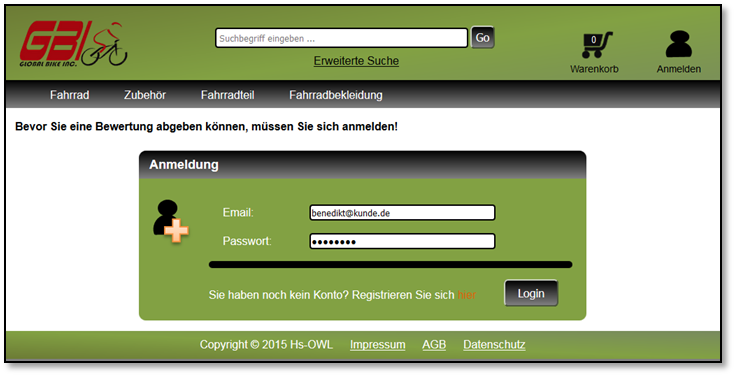
\includegraphics[width=12cm]{Bilder/Michael_Abbildung11-ArtikelBewertenOhneAnmeldung.png}
\end{center}
\caption{Artikel bewerten ohne Anmeldung}
\end{figure}

Ist man im System angemeldet, ist man berechtigt eine Bewertung zu verfassen.
Die Idee der Bewertungsfunktion ist angelehnt an die von Amazon. Der Benutzer muss drei Angaben machen, bevor die Bewertung abgegeben werden kann: Eine Sternbewertung, eine Überschrift und schließlich ein Text bzw. Kommentar. 

\begin{figure}[H]
\begin{center}
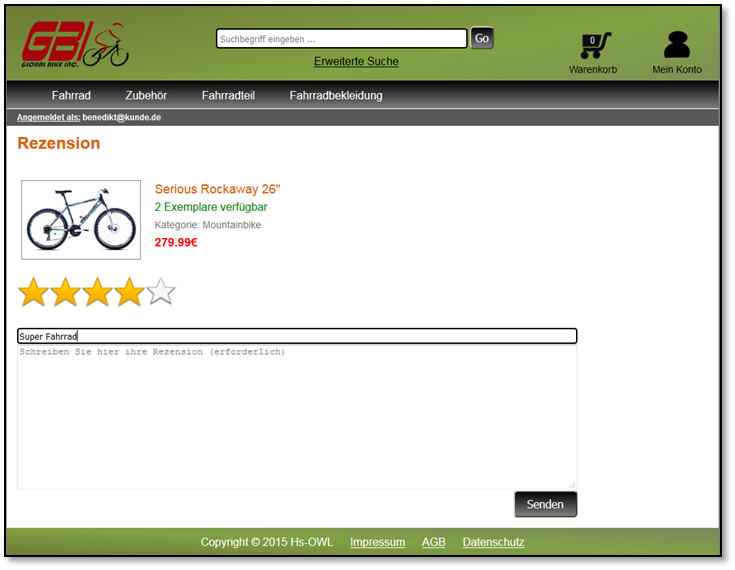
\includegraphics[width=12cm]{Bilder/Michael_Abbildung12-ArtikelBewertenMitAnmeldung.png}
\end{center}
\caption{Artikel bewerten mit Anmeldung}
\end{figure}

\newpage
Wird der Submit-Button geklickt, wird, wie auch bei der Suche oder Registrierung, über JavaScript überprüft, ob die Eingabe gültig ist. Dabei kommt es nicht auf den Inhalt des Geschriebenen an, sondern einfach nur dass alle Felder ausgefüllt sind. Sind alle Angaben gemacht worden, werden die Daten in die Datenbank geladen. Dazu wird die dafür zuständige Methode in der Klasse „Kommentar“ aufgerufen. Es wird sowohl die Produkt-ID als auch die Kunden-ID gespeichert. Das ermöglicht es, alle Bewertungen eines Produktes anzeigen zu lassen, als auch alle Bewertungen eines Kunden. Wenn ein Benutzer einen Artikel bewerten will, welcher schon zuvor von ihm bewertet wurde, wird seine ursprüngliche Bewertung angezeigt. Diese kann er dann nach Belieben ändern.
\\
Der Menüpunkt „Meine Rezensionen“
\\
Dem Benutzer soll es ermöglicht werden, all seine Rezensionen zu verwalten. Dazu wird in dem Menü zur Übersicht der Kontofunktionen ein neuer Menüpunkt erstellt: Meine Rezensionen. 

%\begin{figure}[H]
%\begin{center}
%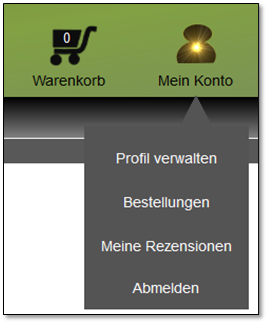
\includegraphics[width=4cm]{Bilder/Michael_Abbildung13-ZusaetzlicherMenuepunkt.png}
%\end{center}
%\caption{Zusätzlicher Menüpunkt}
%\end{figure}

Über diesen Button gelangt der Benutzer auf eine Seite all seiner Rezensionen und kann diese dort ändern oder löschen.

\begin{figure}[H]
\begin{center}
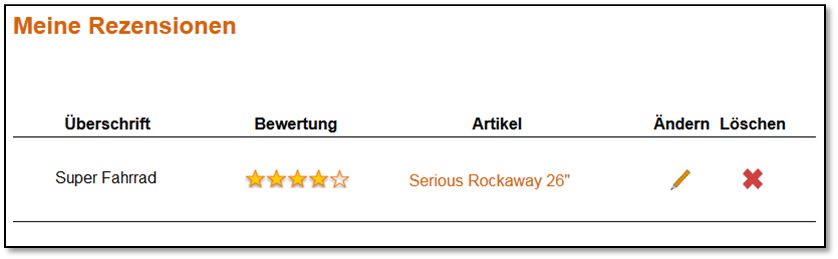
\includegraphics[width=12cm]{Bilder/Michael_Abbildung14-AnzeigeAllerRezensionenEinesBenutzers.png}
\end{center}
\caption{Anzeige aller Rezensionen eines Benutzers}
\end{figure}

\newpage

\subsubsection{Arbeitspaket 12: Die Gestaltung einer Bestätigungs-Email}

Wenn sich ein neuer Benutzer auf der Webseite registriert hat, wird, wie es bei den meisten Online-Shops der Fall ist, eine Bestätigungsmail an die E-Mail-Adresse gesendet, die bei der Registrierung angegeben wird. Dieses Verfahren ist notwendig, um die Korrektheit der E-Mail zu bestätigen. 
Solange die E-Mail vom Benutzer nicht bestätigt wurde, kann der Benutzer sich nicht im GBI-Webshop einloggen. Die Tabelle „kunde“ in der Datenbank enthält eine Spalte „aktiviert“, in die der Status steht. Sobald der Benutzer die E-Mail bestätigt, wird der Kunde aktiviert und kann sich nun im Webshop anmelden.
\\
Vorgehen:
\\
Die E-Mail wird versandt, nachdem die Eingabe bei der Registrierung auf dessen Gültigkeit überprüft worden ist und der Kunde zur Datenbank hinzugefügt wurde. 

%\begin{figure}[H]
%\begin{center}
%
\includegraphics[width=12cm]{Bilder/Michael_Quellcode1.png}
%\end{center}
%\caption{IN QUELLCODE UMWANDELN Klasse Kunde ab Zeile 484!!!}
%\end{figure}

\begin{center}
	\begin{lstinputlisting}[language=PHP, caption={Aktivierungs-E-Mail versenden}]
		{Quellcode/Michael-Quellcode3.php}
	\end{lstinputlisting}
\end{center}

Die Methode \glqq sende\_aktivierungsmail\_registrierung\grqq{} der Klasse \glqq{Kunde}\grqq{} wird aufgerufen. In dieser Methode wird eine Verbindung zu der Datenbank hergestellt, um die Daten des Kunden auszulesen.  Dies ist erforderlich um die E-Mail kundenspezifischer zu gestalten.
Weiter wird der Anredesatz und die E-Mail-Nachricht verfasst.

%\begin{figure}[H]
%\begin{center}
%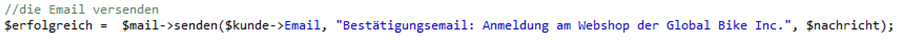
\includegraphics[width=12cm]{Bilder/Michael_Quellcode2.png}
%\end{center}
%\caption{IN QUELLCODE UMWANDELN!!!}
%\end{figure}

\begin{center}
	\begin{lstinputlisting}[language=PHP, caption={Die E-Mail versenden}]
		{Quellcode/Michael-Quellcode4.php}
	\end{lstinputlisting}
\end{center}

\newpage
Anschließend muss die E-Mail nur noch versandt werden.

%\begin{figure}[H]
%\begin{center}
%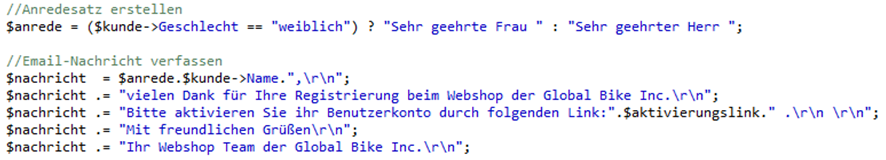
\includegraphics[width=12cm]{Bilder/Michael_Quellcode3.png}
%\end{center}
%\caption{IN QUELLCODE UMWANDELN!!!}
%\end{figure}

\begin{center}
	\begin{lstinputlisting}[language=PHP, caption={Anredesatz erstellen und E-Mail Nachricht verfassen}]
		{Quellcode/Michael-Quellcode5.php}
	\end{lstinputlisting}
\end{center}

Um den Kunden zu aktivieren, befinden sich in der gleichen Klasse die Methode \\
\glqq{aktiviere\_Kunde\_durch\_aktivierungs\_code}\grqq{}. 